% Status Slide --------------------------------------------------------------- %
\begin{frame}{Status}
	\begin{alertblock}{Research Motivation}
	Distributed space systems which include both cooperative and non-cooperative constellations demand autonomous decision making algorithms to manage mission planning, task allocation, and maneuver planning.
		
	\end{alertblock}

	\begin{block}{Completed Work}
		\begin{itemize}
			
			\item \textbf{Central Planner (On Ground)} The task assignment is performed by a central planing algorithm on the ground, which collects information about the satellites and the mission tasks, and then assigns tasks based on the constraints and availabilities of each satellite.
			\item \textbf{Modeling} The system constraints are modelled in Eclipse Modeling Framework to easily manage the mission planning process.
			\item \textbf{Reconfiguration - Ongoing} Simulations for different mission scenarios are performed in order to investigate the possibility of reconfiguration of missions in satellites during run-time.
		\end{itemize}
	\end{block}
\end{frame}

% Future Work Slide ---------------------------------------------------------- %
\begin{frame}{Future Work}
	

	\begin{block}{Future Work}
		\begin{itemize}
			\item \textbf{Decentralized Mission Planning} Developing decentralized decision-making algorithms for satellite constellations. The algorithms will enable satellites to make decisions based on local information and interactions with neighboring satellites, without relying on a central controller. This part aims to design an on-board scheduling algorithm for constellations.
			\item \textbf{Performance Comparison} Comparing the performance of the centralized and distributed algorithms through simulations.
			\item \textbf{Integrating Maneuver Planning} Implementing maneuvering planning for satellites to optimize their positions and orientations in order to execute assigned tasks and avoid collisions. Control algorithms should guarantee that the end state of the satellite is reachable with the scheduled possible maneuvers. 
			\item \textbf{Uncertainty Handling} Examining the impact of uncertainties on self-organization algorithms.
		\end{itemize}
	\end{block}
\end{frame}

\begin{comment}
% First Slide ---------------------------------------------------------------- %
\begin{frame}{Example}
	\framesubtitle{Blocks and Columns}
		\begin{columns}[c]
			\begin{column}{0.45\textwidth}
				\begin{block}{Left Block}
					\begin{itemize}
						\item First Item
						\item[$\rightarrow$] Second
					\end{itemize}
				\end{block}
			\end{column}

			\begin{column}{0.45\textwidth}
				\begin{block}{Right Block}
					\begin{itemize}
						\item First Item
						\item[$\rightarrow$] Second
					\end{itemize}
				\end{block}
			\end{column}
		\end{columns}
\end{frame}


% Second Slide --------------------------------------------------------------- %
\begin{frame}{Example}
	\framesubtitle{Figure}
	\begin{columns}[c]
		\begin{column}{0.45\textwidth}
			\begin{block}{Left Block}
				\begin{itemize}
					\item First Item
					\item[$\rightarrow$] Second
				\end{itemize}
			\end{block}
		\end{column}

		\begin{column}{0.45\textwidth}
			\begin{figure}
				\centering
				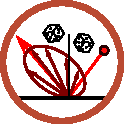
\includegraphics[width=0.8\textwidth]{figures/logos/A02_ring.pdf}
				\caption{Scattering}
			\end{figure}
		\end{column}
	\end{columns}
\end{frame}



% Fourth Slide --------------------------------------------------------------- %
\sectionframeA{The Earth's Atmosphere}{An Introduction to VLEO}

% Fifth Slide ---------------------------------------------------------------- %
\sectionframeB{The Earth's Atmosphere}{An Introduction to VLEO}

% PICLas Slide --------------------------------------------------------------- %
\piclasslide

\end{comment}